\documentclass[
  11pt,
  a4paper,
  % titlepage,
]{article}

\title{Data Structures, Algorithms and Databases}
\author{Martin de Spirlet}
\date{}

% Set document geometry
\usepackage[
  a4paper,
  margin = 1in,
  % showframe,
]{geometry} % Flexible and complete interface to document dimensions

% Set default font family to default sans-serif font
\renewcommand{\familydefault}{\sfdefault}

\usepackage{booktabs} % Publication quality tables in LaTeX
\usepackage[labelfont=bf,labelsep=period]{caption}[2018/05/01] % Customising captions in floating environments
\usepackage[inline,shortlabels]{enumitem} % Control layout of itemize enumerate description
\usepackage{graphicx} % Enhanced support for graphics
\usepackage[skip=\glueexpr\baselineskip\relax]{parskip} % Layout with zero \parindent non-zero \parskip
\usepackage[onehalfspacing]{setspace} % Set space between lines % setspace must be loaded before hyperref
\usepackage{sfmath} % Sans-serif mathematics

% Set list parameters (using enumitem package)
\setlist{nosep}

% Increase penalty for widows and orphans (maximum 10000)
\widowpenalty = 10000
\clubpenalty = 10000

\begin{document}

\pagenumbering{gobble}

\maketitle

\vspace*{\fill}

\begin{table}[htp]
  \centering
  \begin{tabular}{rrl}
    \toprule
    Week & Unit & Title \\
    \midrule
    1 & 1 & Introduction and Entity Relationships \\
    2 & 2 & Functional Dependencies \\
    \bottomrule
  \end{tabular}
\end{table}

\vspace*{\fill}
\addvspace{1in}

\clearpage

\pagenumbering{arabic}

\section{Introduction and Entity Relationships}
\subsection{The Benefits of Databases}

Databases provide
\begin{itemize}
  \item concurrent access for a large number of users,
  \item data integrity,
  \item high throughput and availability,
  \item fault tolerance, and
  \item the ability to store large amounts of structured data.
\end{itemize}

In addition, databases provide abstraction, and allow for the use of bespoke methods of access, such as structured query language (SQL).
Many database management systems (DBMS) make use of variations of SQL.

\subsection{SQL Tables}

SQL operates on \emph{tables}.
A table is the implementation of a \emph{relation} --- a theoretical construct with certain properties.
The rows of a table correspond to the \emph{tuples} of a relation.
The columns of a table correspond the the \emph{attributes} of a relation.

A relation is a \emph{set} of tuples.
Although a table may contain duplicate rows, a relation may not contain duplicate tuples.
Additionally, the way in which data is stored implies that tables are ordered in some way.
This is not the case for relations.

\begin{table}[htp]
  \centering
  \caption*{A table in SQL.}
  \begin{tabular}{rlr}
    \toprule
    id & name & mark \\
    \midrule
    1 & Alice & 90 \\
    2 & Bob & 80 \\
    3 & Charlotte & 70 \\
    4 & David & 60 \\
    \bottomrule
  \end{tabular}
\end{table}

The schema of a table is the logical definition of a table.
This includes the number of columns (attributes), their names and the type of information they store.

\subsection{Normalisation}

Storing all information in a single table leads to redundancy.
This can be avoided by \emph{normalising} tables --- linking information across multiple tables.

\subsection{Constraints}

SQL provides a way of imposing certain rules (\emph{constraints}) to tables.
Constraints include \texttt{NOT~NULL}, \texttt{UNIQUE}, \texttt{PRIMARY~KEY}, \texttt{FOREIGN~KEY}, \texttt{CHECK}, \texttt{DEFAULT} and \texttt{INDEX}.
A \emph{primary~key} is a set of attributes that uniquely identify a row.

\subsection{Database Design Goals}

A database design must
\begin{itemize}
  \item work within predefined business rules,
  \item ensure data consistency and throughput,
  \item contain all the required data, and
  \item ensure that the data remains readable despite these constraints.
\end{itemize}

Examples of business rules include
\begin{itemize}
  \item an order must be placed before it is shipped, and
  \item the timetables for a single student must not overlap.
\end{itemize}
These business rules can be implemented using database constraints.
Having the correct information with the required constraints constitutes \emph{data~quality}, which is critical to the smooth operation of an organisation.
Nevertheless, having all this required information in a database is not so useful if the database is too slow.
A balance must be struck between business requirements and throughput.

\subsection{Entity Relationship Diagrams}

\subsubsection{Crow's Feet Notation}

Entity relationship diagrams (ERDs) are a notation for database design.
There is no standard for (ERDs), but one popular family of notation is \emph{Crow's~Feet Notation}.

\subsubsection{Entities and Relationships}

Commonly, an entity is denoted by a rectangle.
An entity often represent nouns, such as objects or events.
The relationship between two entities is written on a line connecting them.
The relationship is usually a verb.
Thus, ERDs correspond to natural language.

\begin{figure}[htp]
  \centering
  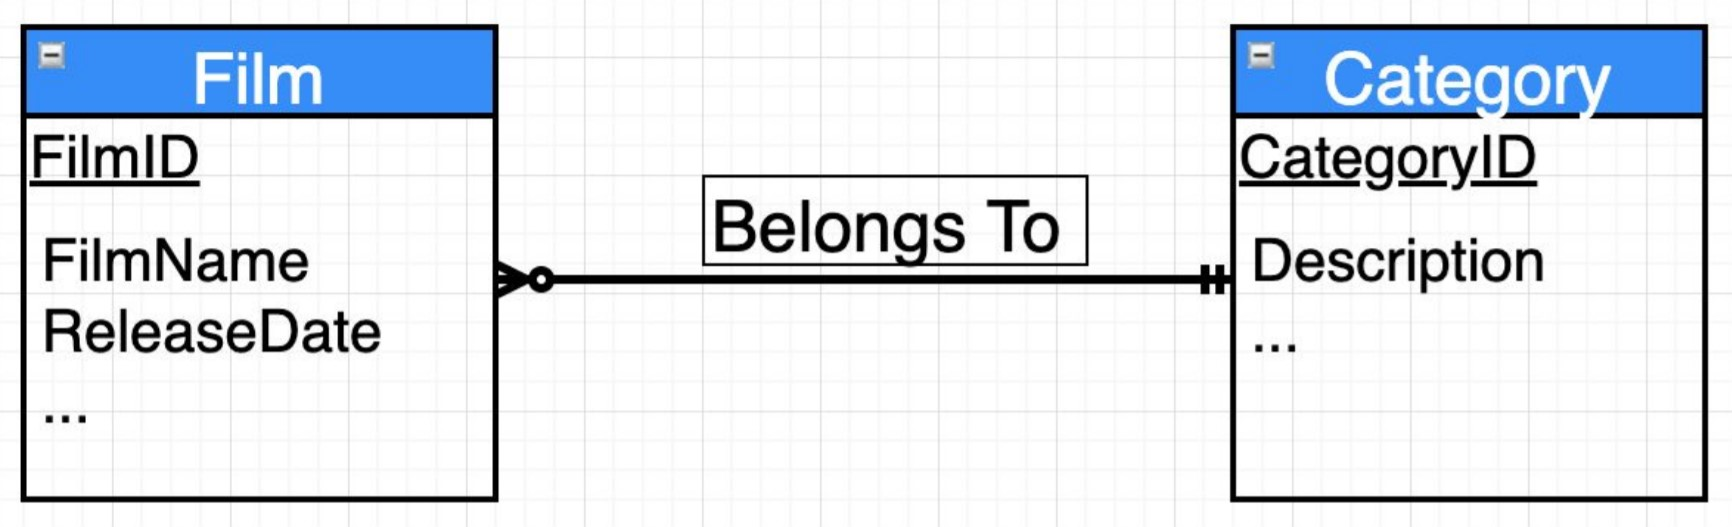
\includegraphics[width=0.75\textwidth]{unit-1/figures/er-diagram.jpg}
  \caption*{An entity relationship diagram.}
\end{figure}

The attributes of an entity are listed within its rectangle.
The primary key is underlined.

Relationships are named associations between entities.
Relationships provide associations in both directions.

\subsubsection{Cardinality}

\emph{Cardinality} provides a constraint on the number of instances of an entity that participate in a relationship.

\begin{figure}[htp]
  \centering
  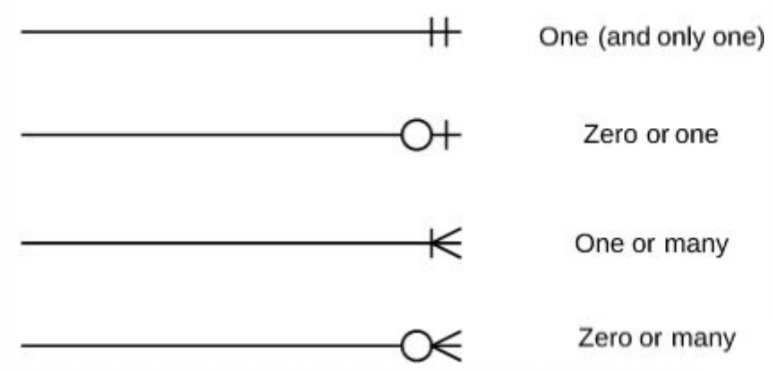
\includegraphics[width=0.6\textwidth]{unit-1/figures/cardinality-notation.jpg}
  \caption*{Cardinality notation.}
\end{figure}

\begin{table}[htp]
  \centering
  \caption*{Important cardinalities.}
  \begin{tabular}{ll}
    \toprule
    Name & Value \\
    \midrule
    Mandatory & Minimum cardinality \( \geq 1 \) \\ [1ex]
    Optional & Minimum cardinality \( = 0 \) \\ [1ex]
    Functional & Minimum cardinality \( = 1 \) \\ [1ex]
    \midrule
    One-to-one (1--1) & Maximum cardinality \( = 1 \) in both directions \\ [1ex]
    One-to-many (1--M) & Maximum cardinality \( = 1 \) in one direction \\
    & Maximum cardinality \( > 1 \) in the other direction \\ [1ex]
    Many-to-many (M--N) & Maximum cardinality \( > 1 \) in both directions \\
    \bottomrule
  \end{tabular}
\end{table}

\subsubsection{Foreign Keys and Weak Entities}

Relationships are translated to \emph{foreign~keys} in tables, except in the case of many-to-many relationships.

\emph{Weak~entities} are entities that do not have their own primary~key.
They must borrow attributes from other entities to form part or all of their primary~key.
Weak~entities are represented by rounded rectangles.
An underlined attribute of a weak~entity is not its primary key.
It is a key that is combined with the keys of one or more entities to provide a primary key.

\begin{figure}[htp]
  \centering
  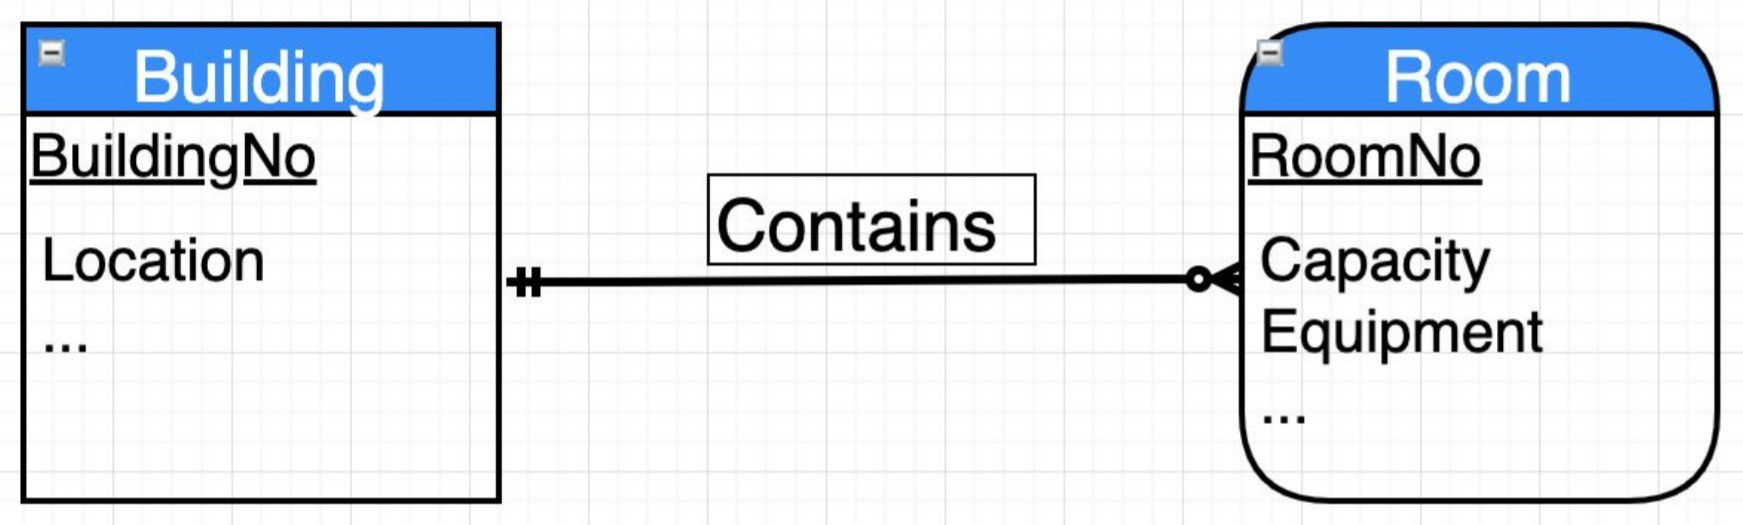
\includegraphics[width=0.75\textwidth]{unit-1/figures/weak-entity.jpg}
  \caption*{A weak entity relationship.}
\end{figure}

An \emph{identification relationship} provides one component of the primary key of a weak entity.
An \emph{identifying dependency} consists of one or more identification relationships that provide all of the primary key.
Sometimes an identification relationship and an identifying dependency are equivalent.

\subsubsection{Many-to-Many Relationships}

In a many-to-many relationship, the relationship itself can have attributes.
Theses attributes are listed below the relationship with an arrow pointing to them.

\begin{figure}[htp]
  \centering
  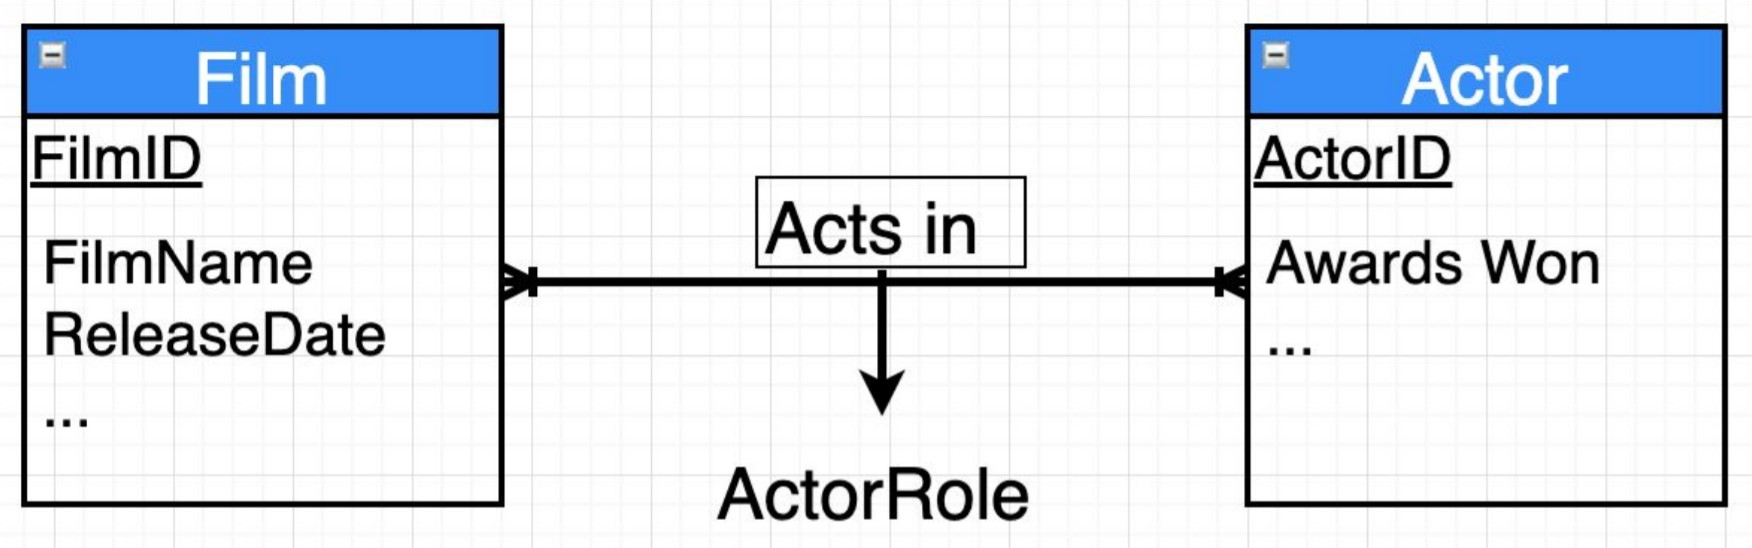
\includegraphics[width=0.75\textwidth]{unit-1/figures/relationship-attribute.jpg}
  \caption*{An attribute of a many-to-many relationship.}
\end{figure}

A many-to-many relationship can be replaced by an associate entity and two one-to-many relationships.

\begin{figure}[htp]
  \centering
  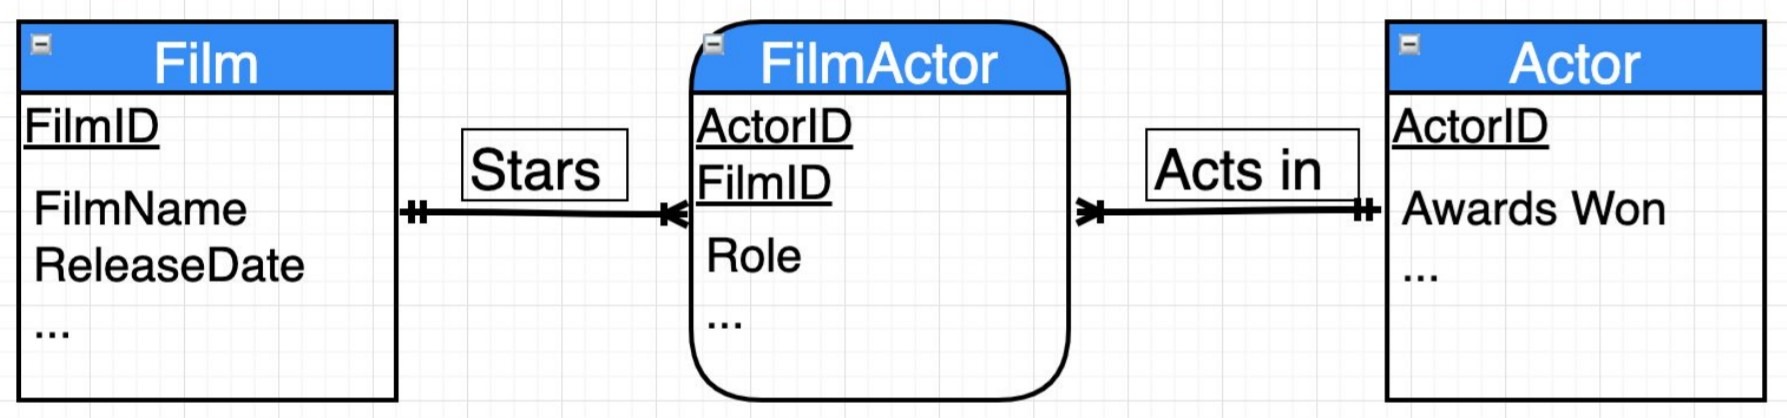
\includegraphics[width=\textwidth]{unit-1/figures/associate-entity.jpg}
  \caption*{An associate entity in a many-to-many relationship.}
\end{figure}

An associate entity provides additional information about the many-to-many relationship it implements.
By necessity, an associate entity is a weak entity that borrows the attributes of its primary~key from the entities between which it provides an association.

\subsubsection{\texorpdfstring{\( N \)}{N}-Way Relationships}

Sometimes --- though very rarely --- more than two entities are related to each other.
For example, a module may be taught by multiple lecturers, and a student is given a mark from each lecturer.
If it is only necessary to relate pairs of entities, such as which lecturers teach which modules, or which students are enrolled in which modules, an \( N \)-way relationship is not required.
If, however, it is necessary to store information associated with more than two entities, such as the mark given to a student from a lecturer for one section of a module, an \( N \)-way relationship is required.

\begin{figure}[htp]
  \centering
  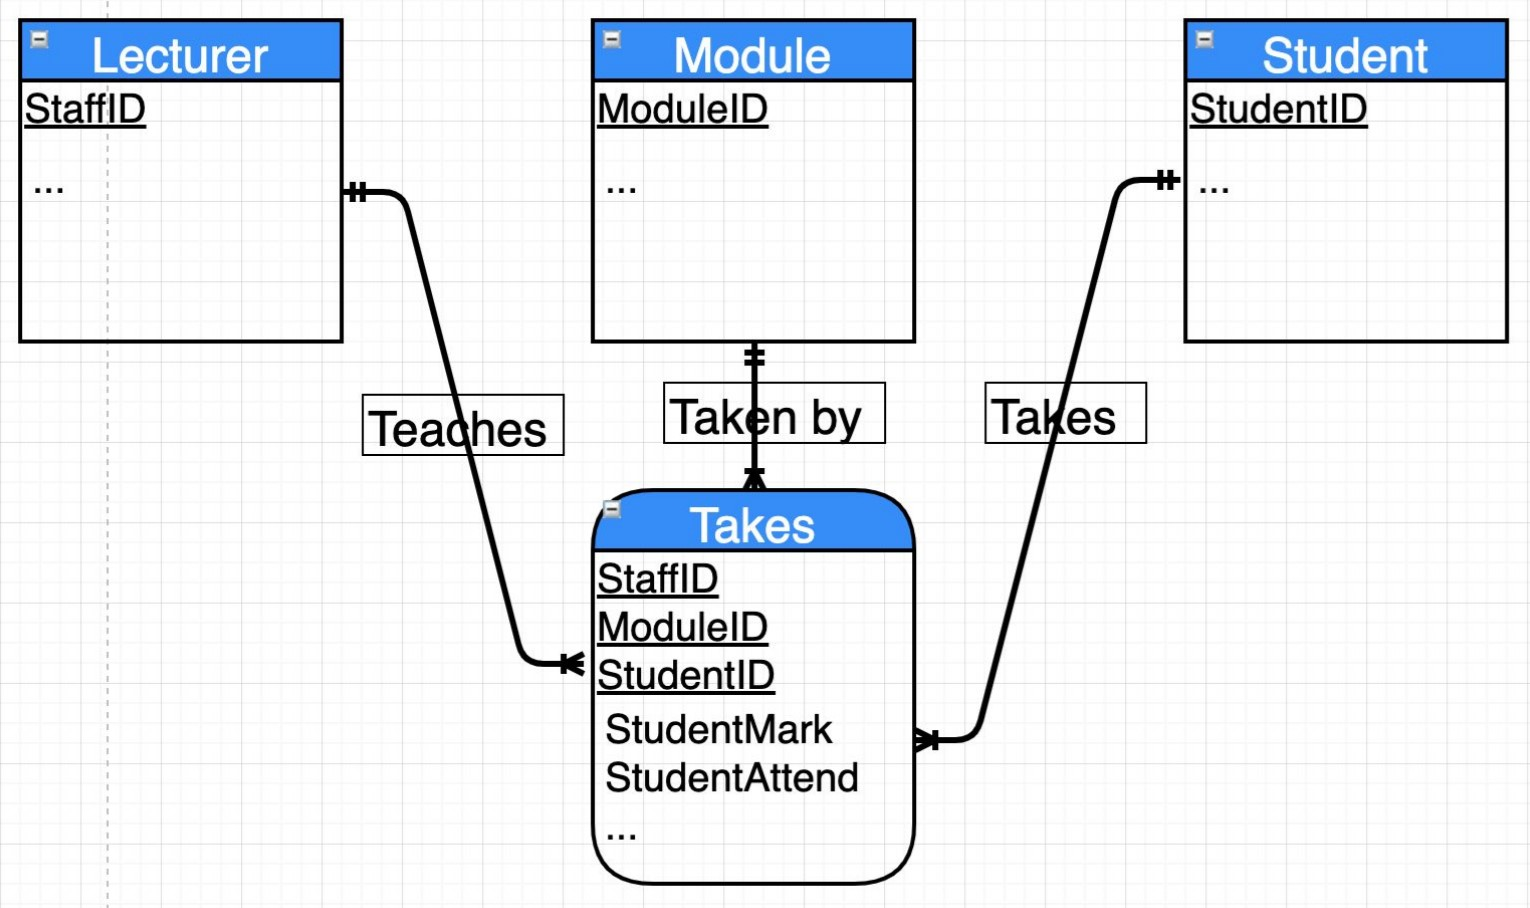
\includegraphics[width=\textwidth]{unit-1/figures/n-way-relationship.jpg}
  \caption*{An \( N \)-way relationship.}
\end{figure}

\subsubsection{Self-Identifying Relationships}

A \emph{self-identifying} (also \emph{self-referencing} or \emph{reflexive}) relationship is a relationship between an entity and itself.

\begin{figure}[htp]
  \centering
  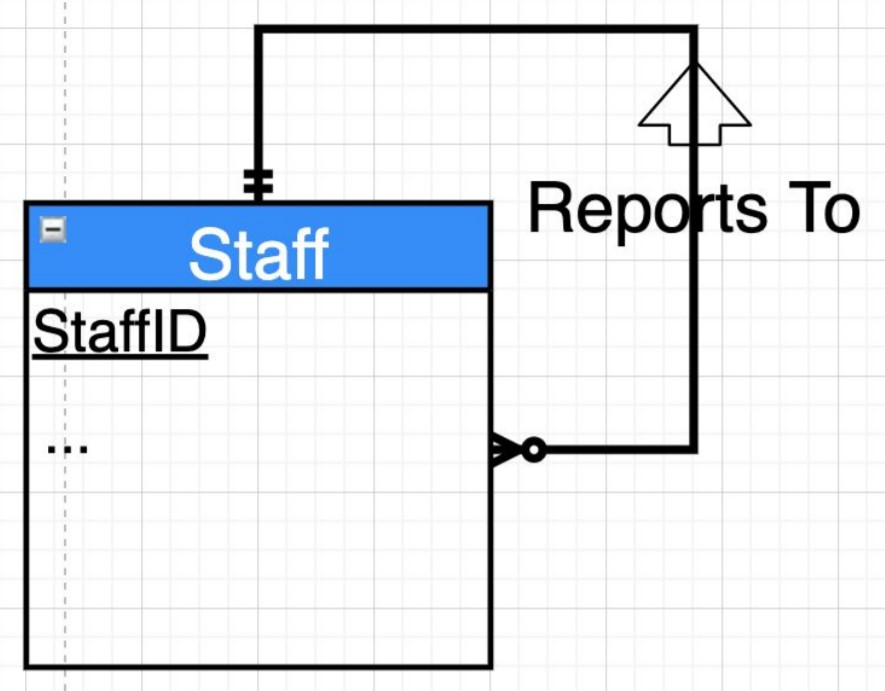
\includegraphics[width=0.4\textwidth]{unit-1/figures/self-identifying-relationship.jpg}
  \caption*{A self-identifying relationship.}
\end{figure}

All hierarchies are self-identifying relationships.
\begin{itemize}
  \item Biological classifications
  \item Organisational hierarchies
  \item Topic categories
\end{itemize}

In order to determine the cardinality of a self-identifying relationship, it is useful to draw an \emph{instance~diagram}.

\begin{figure}[htp]
  \centering
  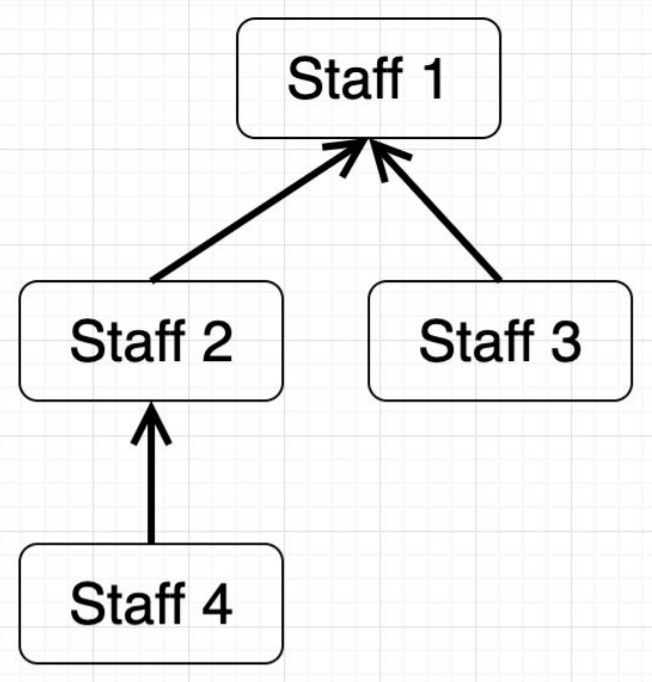
\includegraphics[width=0.3\textwidth]{unit-1/figures/instance-diagram.jpg}
  \caption*{An instance diagram of a self-identifying relationship.}
\end{figure}

A self-identifying relationship may require an associate entity, depending on its cardinality.
All self-identifying relationships can be translated to tables if many-to-many relationships are replaced by associate entities and one-to-many relationships.


\section{Functional Dependencies}
\subsection{Relational Design by Decomposition}

In its simplest form, all data could be stored in one large table with several columns.
The problem with this is that
\begin{itemize}
  \item the redundancy in repeated data will lead to a tremendous waste of space, and
  \item the throughput and availability of the data is diminished by the size of the table.
\end{itemize}

Instead, the large table is \emph{decomposed} into several smaller tables.

\subsection{Functional Dependency Notation}

\emph{Functional~dependencies} are a generalisation of keys.
The functional dependencies of a relation are based on knowledge of the real world.
All instances of the relation must adhere to its functional dependencies.

\begin{table}[htp]
  \centering
  \caption*{Attributes of the \emph{students} relation.}
  \begin{tabular}{llllllll}
    \toprule
    sID & sName & sAddress & fdUniCode & fdUniName & fdUniCity & fdUniMark & fdGrade \\
    \bottomrule
  \end{tabular}
\end{table}

Suppose that the `fdGrade' attribute of the students relation is based on the corresponding `fdMark'.
For example, a mark of 70 may map to a grade of A, and a mark of 60 may map to a grade of B\@.
It can be said that `fdGrade' is \emph{functionally~determined} by `fdMark', or `fdMark' \emph{functionally~determines} `fdGrade'.
In other words, any two tuples with the same `fdMark' must have the same `fdGrade'.
\begin{equation*}
  \text{fdMark} \rightarrow \text{fdGrade}
\end{equation*}

For every pair of tuples \( t \) and \( u \) that are elements of the student relation, the equality of the `fdMark' of both tuples implies the equality of the `fdGrade' of both tuples.
\begin{equation*}
  \forall\ t,u \in \text{students}: \quad t.\text{fdMark} = u.\text{fdMark} \implies t.\text{fdGrade} = u.\text{fdGrade}
\end{equation*}

In general, the functional dependency by which a set of attributes \( \itol{A} = \left\{ a_1, a_2, \ldots, a_m \right\} \) functionally determines a set of attributes \( \itol{B} = \left\{ b_1, b_2, \ldots, b_n \right\} \) in a relation \( R \) is defined as
\begin{equation*}
  \itol{A} \rightarrow \itol{B}
\end{equation*}
\begin{equation*}
  \forall\ t,u \in R: \quad t.\itol{A} = u.\itol{A} \implies t.\itol{B} = u.\itol{B}
\end{equation*}

\subsection{Interpreting Functional Dependencies}

The student~ID uniquely identifies a student; no two students can have the same ID\@.
\begin{equation*}
  \text{sID} \rightarrow \text{sName}
\end{equation*}

The student~ID uniquely identifies the registered address; a student cannot be registered under two addresses.
\begin{equation*}
  \text{sID} \rightarrow \text{sAddress}
\end{equation*}

The first~degree university~code uniquely identifies the name and city of the university; no two universities can have the same university~code.
\begin{equation*}
  \text{fdUniCode} \rightarrow \text{fdUniName}, \text{fdUniCity}
\end{equation*}

The name and city of a university uniquely identifies the university; no two universities in the same city can have the same name.
\begin{equation*}
  \text{fdUniName}, \text{fdUniCity} \rightarrow \text{fdUniCode}
\end{equation*}

The student~ID uniquely identifies the first~degree mark of the student with that ID; a student can only have one first~degree mark.
\begin{equation*}
  \text{sID} \rightarrow \text{fdMark}
\end{equation*}

The first~degree mark determines the first~degree grade; any two students with the same mark must have the same grade.
\begin{equation*}
  \text{fdMark} \rightarrow \text{fdGrade}
\end{equation*}

The student~ID uniquely identifies the first~degree grade of the student with that ID; a student can only have one first~degree grade.
\begin{equation*}
  \text{sID} \rightarrow \text{fdGrade}
\end{equation*}

\subsection{Functional Dependencies and Keys}

A key is a set of attributes that uniquely identifies a tuple.
If a set of attributes \( \itol{A} \) functionally determines all attributes of a relation \( R \) with no duplicates, then \( \itol{A} \) is a key of \( R \)\@.

\subsection{Types of Functional Dependency}

\subsubsection{Trivial Dependencies}

A functional dependency \( \itol{A} \rightarrow \itol{B} \) is said to be a \emph{trivial} functional dependency if \( \itol{B} \) is a subset of \( \itol{A} \).
\begin{equation*}
  \itol{A} \rightarrow \itol{B} \quad \text{is trivial if} \quad \itol{B} \subseteq \itol{A}
\end{equation*}

\subsubsection{Non-Trivial Dependencies}

A functional dependency \( \itol{A} \rightarrow \itol{B} \) is said to be a \emph{non-trivial} functional dependency if \( \itol{B} \) is \emph{not} a subset of \( \itol{A} \)\@.
\begin{equation*}
  \itol{A} \rightarrow \itol{B} \quad \text{is non-trivial if} \quad \itol{B} \nsubseteq \itol{A}
\end{equation*}

\subsubsection{Completely Non-Trivial Dependencies}

A functional dependency \( \itol{A} \rightarrow \itol{B} \) is said to be a \emph{completely non-trivial} functional dependency if \( \itol{A} \) and \( \itol{B} \) are disjoint, i.e.\ they share no common attributes --- their intersection is the empty set \( \varnothing \).
\begin{equation*}
  \itol{A} \rightarrow \itol{B} \quad \text{is completely non-trivial if} \quad \itol{A} \cap \itol{B} = \varnothing
\end{equation*}

\subsection{Rules of Functional Dependencies}

\subsubsection{The Splitting Rule}

The \emph{splitting rule} states that if
\begin{equation*}
  \itol{A} \rightarrow b_1, b_2, \ldots, b_n
\end{equation*}
then it follows that
\begin{equation*}
  \itol{A} \rightarrow b_1, \quad \itol{A} \rightarrow b_2, \quad \ldots, \quad \itol{A} \rightarrow b_n
\end{equation*}

\subsubsection{The Combining Rule}

The \emph{combining rule} states that if
\begin{equation*}
  \itol{A} \rightarrow b_1, \quad \itol{A} \rightarrow b_2, \quad \ldots, \quad \itol{A} \rightarrow b_n
\end{equation*}
then it follows that
\begin{equation*}
  \itol{A} \rightarrow b_1, b_2, \ldots, b_n
\end{equation*}

\subsubsection{The Transitive Rule}

The \emph{transitive rule} states that if
\begin{equation*}
  \itol{A} \rightarrow \itol{B} \quad \text{and} \quad \itol{B} \rightarrow \itol{C}
\end{equation*}
then it follows that
\begin{equation*}
  \itol{A} \rightarrow \itol{C}
\end{equation*}

\subsubsection{Trivial Dependency Rules}

If \( \itol{A} \rightarrow \itol{B} \) is a trivial dependency, then \( \itol{A} \) functionally determines the union of \( \itol{A} \) and \( \itol{B} \)\@.
\begin{equation*}
  \itol{B} \subseteq \itol{A} \implies \itol{A} \rightarrow \itol{A} \cup \itol{B}
\end{equation*}

If \( \itol{A} \rightarrow \itol{B} \) is a trivial dependency, then \( \itol{A} \) functionally determines the intersection of \( \itol{A} \) and \( \itol{B} \).
\begin{equation*}
  \itol{B} \subseteq \itol{A} \implies \itol{A} \rightarrow \itol{A} \cap \itol{B}
\end{equation*}

\subsection{Closure of Attributes}

The closure of a set of attributes \( \itol{A} \) in a relation is the set of all attributes \( \itol{B} \) such that \( \itol{A} \rightarrow \itol{B} \)\@.
The closure of \( \itol{A} \) is denoted by \( \itol{A}^{+} \)\@.
Since \( \itol{A} \) is a subset of itself, the closure of \( \itol{A} \) contains \( \itol{A} \)\@.
\begin{equation*}
  \itol{A} \subseteq \itol{A} \quad \therefore \quad \itol{A}^{+} \supseteq \itol{A}
\end{equation*}

In order to determine the closure of \( \itol{A} \),
\begin{enumerate}
  \item define a result set \( \itol{A}^{+} \) that initially contains all attributes of \( \itol{A} \), then
  \item repeating until there is no further change,
  \begin{enumerate}
    \item for all the (remaining) functional dependencies of the form \( \itol{X} \rightarrow \itol{Y} \),
    \begin{enumerate}
      \item if \( \itol{X} \) is a subset of the result set \( \itol{A}^{+} \),
      \begin{enumerate}
        \item add \( \itol{Y} \) to the result set \( \itol{A}^{+} \), and
        \item remove the functional dependency from the list of functional dependencies that remain to be considered.
      \end{enumerate}
    \end{enumerate}
  \end{enumerate}
  \item Finally, the result set \( \itol{A}^{+} \) should be the closure of \( \itol{A} \)\@.
\end{enumerate}

\subsection{Closure, Keys and Decomposition}

To check whether \( \itol{A} \) is a key of a relation \( R \), it is necessary to compute the closure of \( \itol{A} \)\@.
If the closure contains all attributes of \( R \), then \( \itol{A} \) is a key of \( R \)\@.

In general, to find all the keys for a relation \( R \), it is necessary to compute the closure of each and every subset \( \itol{A} \) of the attributes of \( R \)\@.
If the closure of the subset \( \itol{A} \) contains all attributes of \( R \), then \( \itol{A} \) is a key of \( R \)\@.
The problem can be simplified by noting that a superset of a key is itself a key.
Therefore, if a key \( \itol{A} \) is found, all supersets of \( \itol{A} \) can be marked as keys without having to compute their closures.

The purpose of decomposition is to find a minimal set of completely non-trivial functional dependencies such that all functional dependencies that hold on the original relation can be derived from this set.


\end{document}
